%%%%%%%%%%%%%%%%%%%%%%%%%%%%%%%%%%%%%%%%%
% Simple Sectioned Essay Template
% LaTeX Template
%
% This template has been downloaded from:
% http://www.latextemplates.com
%
% Note:
% The \lipsum[#] commands throughout this template generate dummy text
% to fill the template out. These commands should all be removed when 
% writing essay content.
%
%%%%%%%%%%%%%%%%%%%%%%%%%%%%%%%%%%%%%%%%%

%----------------------------------------------------------------------------------------
%	PACKAGES AND OTHER DOCUMENT CONFIGURATIONS
%----------------------------------------------------------------------------------------

\documentclass[12pt]{article} % Default font size is 12pt, it can be changed here
\usepackage{hyperref}

\usepackage{geometry} % Required to change the page size to A4
\geometry{a4paper} % Set the page size to be A4 as opposed to the default US Letter

\usepackage{graphicx} % Required for including pictures

\usepackage{float} % Allows putting an [H] in \begin{figure} to specify the exact location of the figure
\usepackage{wrapfig} % Allows in-line images such as the example fish picture

\usepackage{lipsum} % Used for inserting dummy 'Lorem ipsum' text into the template

\linespread{1.2} % Line spacing

%\setlength\parindent{0pt} % Uncomment to remove all indentation from paragraphs

\graphicspath{{Pictures/}} % Specifies the directory where pictures are stored

\begin{document}

%----------------------------------------------------------------------------------------
%	TITLE PAGE
%----------------------------------------------------------------------------------------

\begin{titlepage}

\newcommand{\HRule}{\rule{\linewidth}{0.5mm}} % Defines a new command for the horizontal lines, change thickness here

\center % Center everything on the page

\textsc{\LARGE Colah's Blog}\\[1.5cm] % Name of your university/college
%\textsc{\Large Christopher Olan}\\[0.5cm] % Major heading such as course name
%\textsc{\large Minor Heading}\\[0.5cm] % Minor heading such as course title

\HRule \\[0.4cm]
{ \huge \bfseries Understanding LSTM Networks}\\[0.4cm] % Title of your document
\HRule \\[1.5cm]

\begin{minipage}{0.4\textwidth}
\begin{flushleft} \large
\emph{Author:}\\
Christopher \textsc{Olan} % Your name
\end{flushleft}
\end{minipage}
~
\begin{minipage}{0.4\textwidth}
\begin{flushright} \large
%\emph{Supervisor:} \\
%Dr. James \textsc{Smith} % Supervisor's Name
\end{flushright}
\end{minipage}\\[4cm]

{\large August 27, 2015}\\[3cm] % Date, change the \today to a set date if you want to be precise

%\includegraphics{Logo}\\[1cm] % Include a department/university logo - this will require the graphicx package

\vfill % Fill the rest of the page with whitespace

\end{titlepage}

%----------------------------------------------------------------------------------------
%	TABLE OF CONTENTS
%----------------------------------------------------------------------------------------

\tableofcontents % Include a table of contents

\newpage % Begins the essay on a new page instead of on the same page as the table of contents 

%----------------------------------------------------------------------------------------
%	INTRODUCTION
%----------------------------------------------------------------------------------------

\section{Recurrent Neural Networks} % Major section

%Example citation \cite{Figueredo:2009dg}. 引用

Humans don't start their thinking from scratch every second. As you read this essay, you understand each word based on your understanding of previous words. You don't throw everything away and start thinking from scratch again. Your thoughts have persistence.

Traditional neural networks can't do this, and it seems like a major shortcoming. For example, imagine you want to classify what kind of event is happening at every point in a movie. It's unclear how a traditional neural network could use its reasoning about previous events in the film to inform later ones.

Recurrent neural networks address this issue. They are networks with loops in them, allowing information to persist.
\begin{figure}[H] % Example image
\center{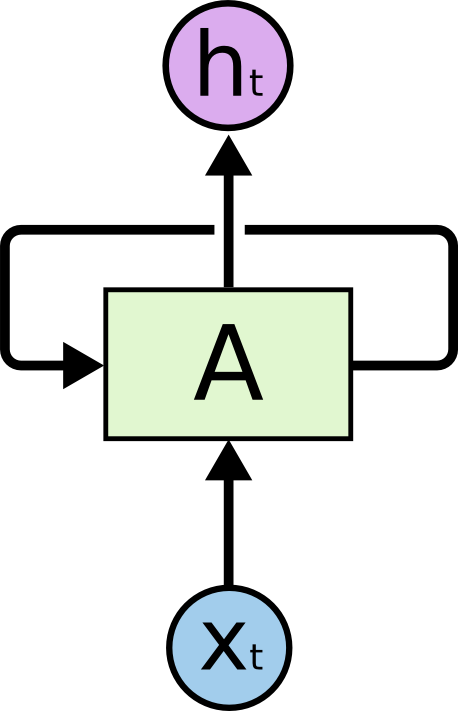
\includegraphics[width=0.38\textwidth]{RNN-rolled}}
\caption{Recurrent Neural Networks have loops.}
\label{fig:recurrentneuralnetworkshaveloops}
\end{figure}

In the above diagram, a chunk of neural network, $A$, looks at some input $x_{i}$ and outputs a value $h_{i}$. A loop allows information to be passed from one step of the network to the next.

These loops make recurrent neural networks seem kind of mysterious. However, if you think a bit more, it turns out that they aren't all that different than a normal neural network. A recurrent neural network can be thought of as multiple copies of the same network, each passing a message to a successor. Consider what happens if we unroll the loop: %就一层
\begin{figure}[H] % Example image
\center{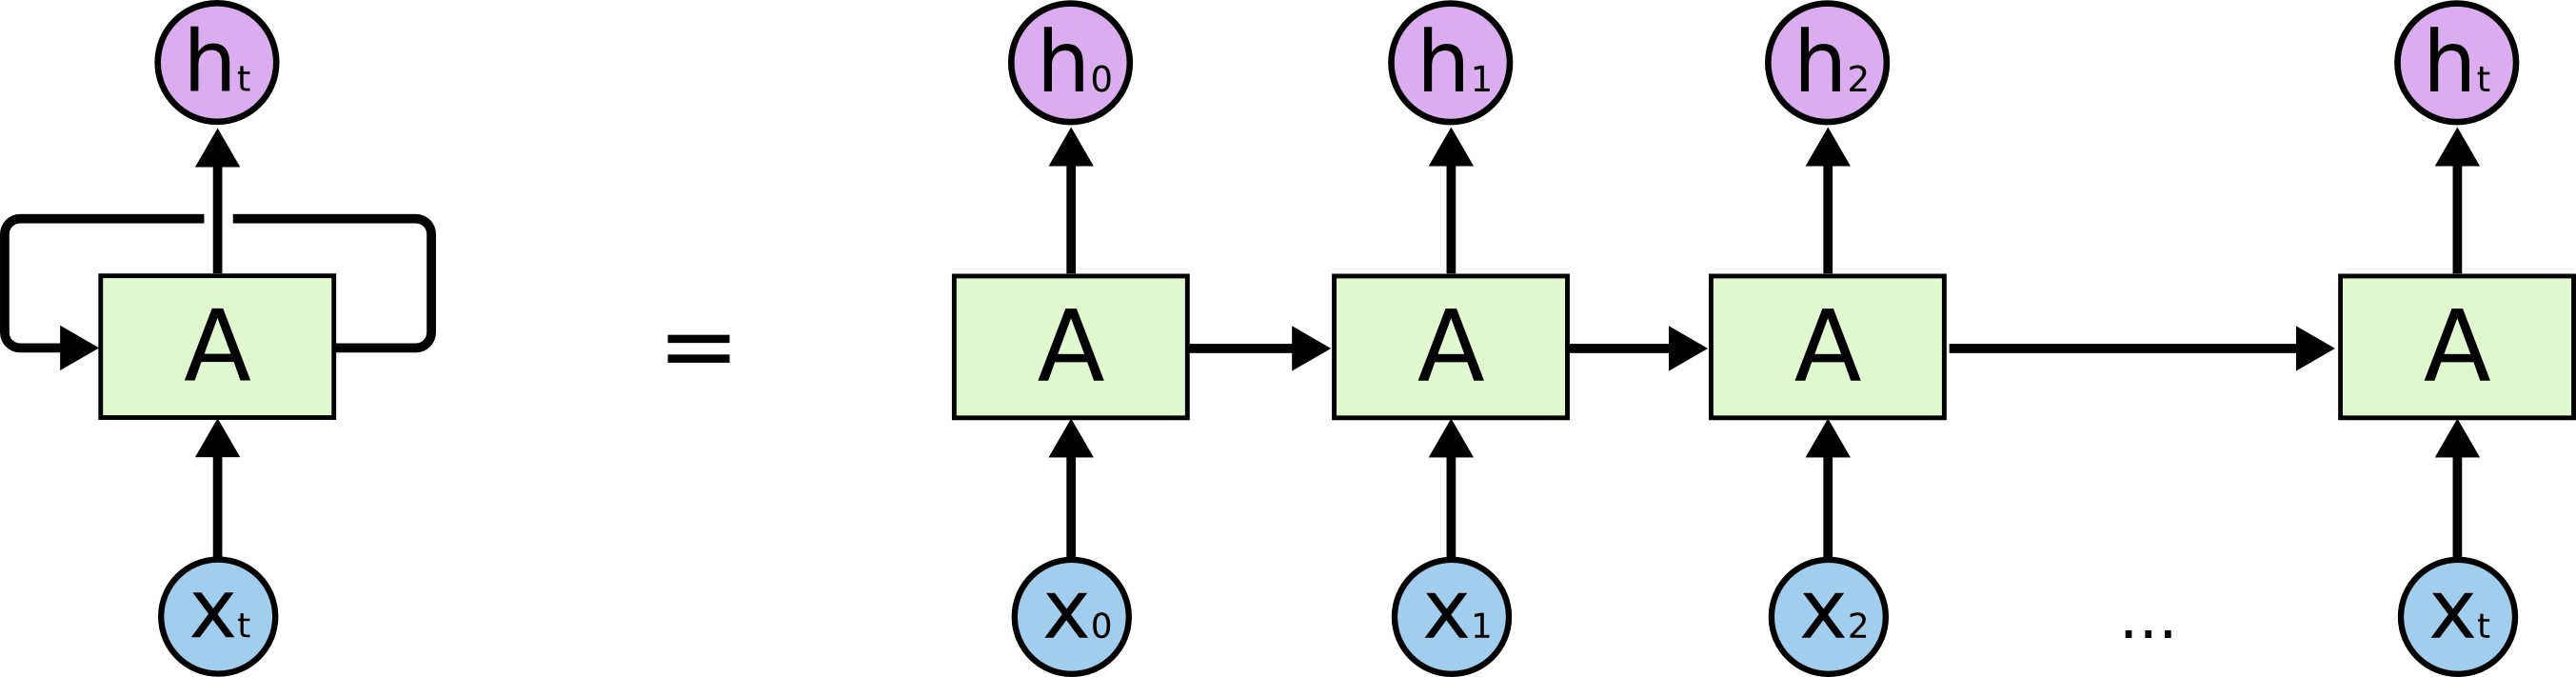
\includegraphics[width=0.9\textwidth]{RNN-unrolled}}
\caption{An unrolled recurrent neural network.}
\label{fig:rnnunrolled}
\end{figure}

This chain-like nature reveals that recurrent neural networks are intimately related to $\textit{sequence and lists}$. They're the natural architecture of neural network to use for such data.

And they certainly are used! In the last few years, there have been incredible success applying RNNs to a variety of problems: speech recognition, language modeling, translation, image captioning... The list goes on. I'll leave discussion of the amazing feats one can achieve with RNNs to Andrej Karpathy's excellent blog post, The Unreasonable Effectiveness of Recurrent Neural Networks\footnote{\url{http://karpathy.github.io/2015/05/21/rnn-effectiveness/}}. But they really are pretty amazing.

Essential to these successes is the use of ``LSTMs,'' a very special kind of recurrent neural network which works, for many tasks, much much better than the standard version. Almost all exciting results based on recurrent neural networks are achieved with them. It's these LSTMs that this essay will explore.

\section{The Problem of Long-Term Dependencies}

One of the appeals of RNNs is the idea that they $might$ be able to connect previous information to the present taks, such as using previous video frames might inform the understanding of the present frame. If RNNs could do this, they'd be extremely useful. But can they? It depends.

Sometimes, we only need to look at recent information to perform the present task. For example, consider a language model trying to predict the next word based on the previous ones. If we are trying to predict the last word in ``the clouds are in the $sky$,'' we don't need any further context---it's pretty obvious the next word is going to be sky. In such cases, where the gap between the revelant information and the place that it's needed is small, RNNs can learn to use the past information.

\begin{figure}[H] % Example image
\center{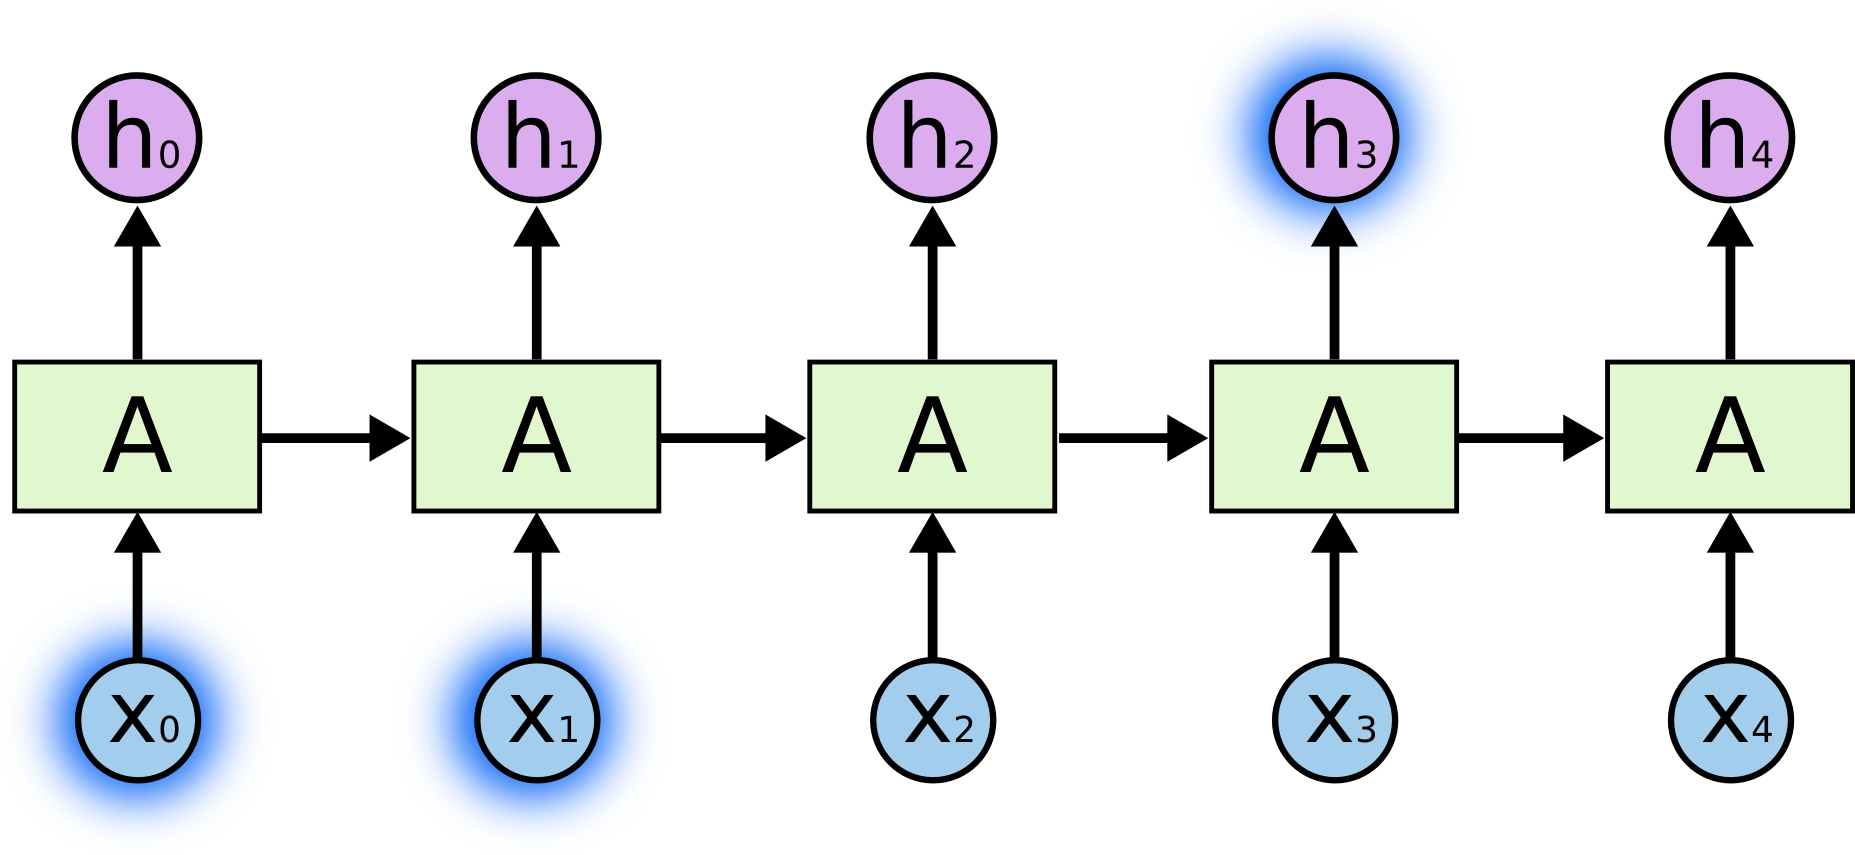
\includegraphics[width=0.9\textwidth]{RNN-shorttermdepdencies}}
%\caption{An unrolled recurrent neural network.}
\label{fig:rnnunrolled}
\end{figure}

But there are also cases where we need more context. Consider trying to predict the last word in the text ``I grew up in France...I speak fluent $French$,'' but if we want to narrow down which language, we need the context of France, from further back. It's entirely possible for the gap between the revelant information and the point where it is needed to become very large.

Unformately, as that gap grows, RNNs become unable to learn to connect the information.
%RNN-longtermdependencies.png
\begin{figure}[H] % Example image
\center{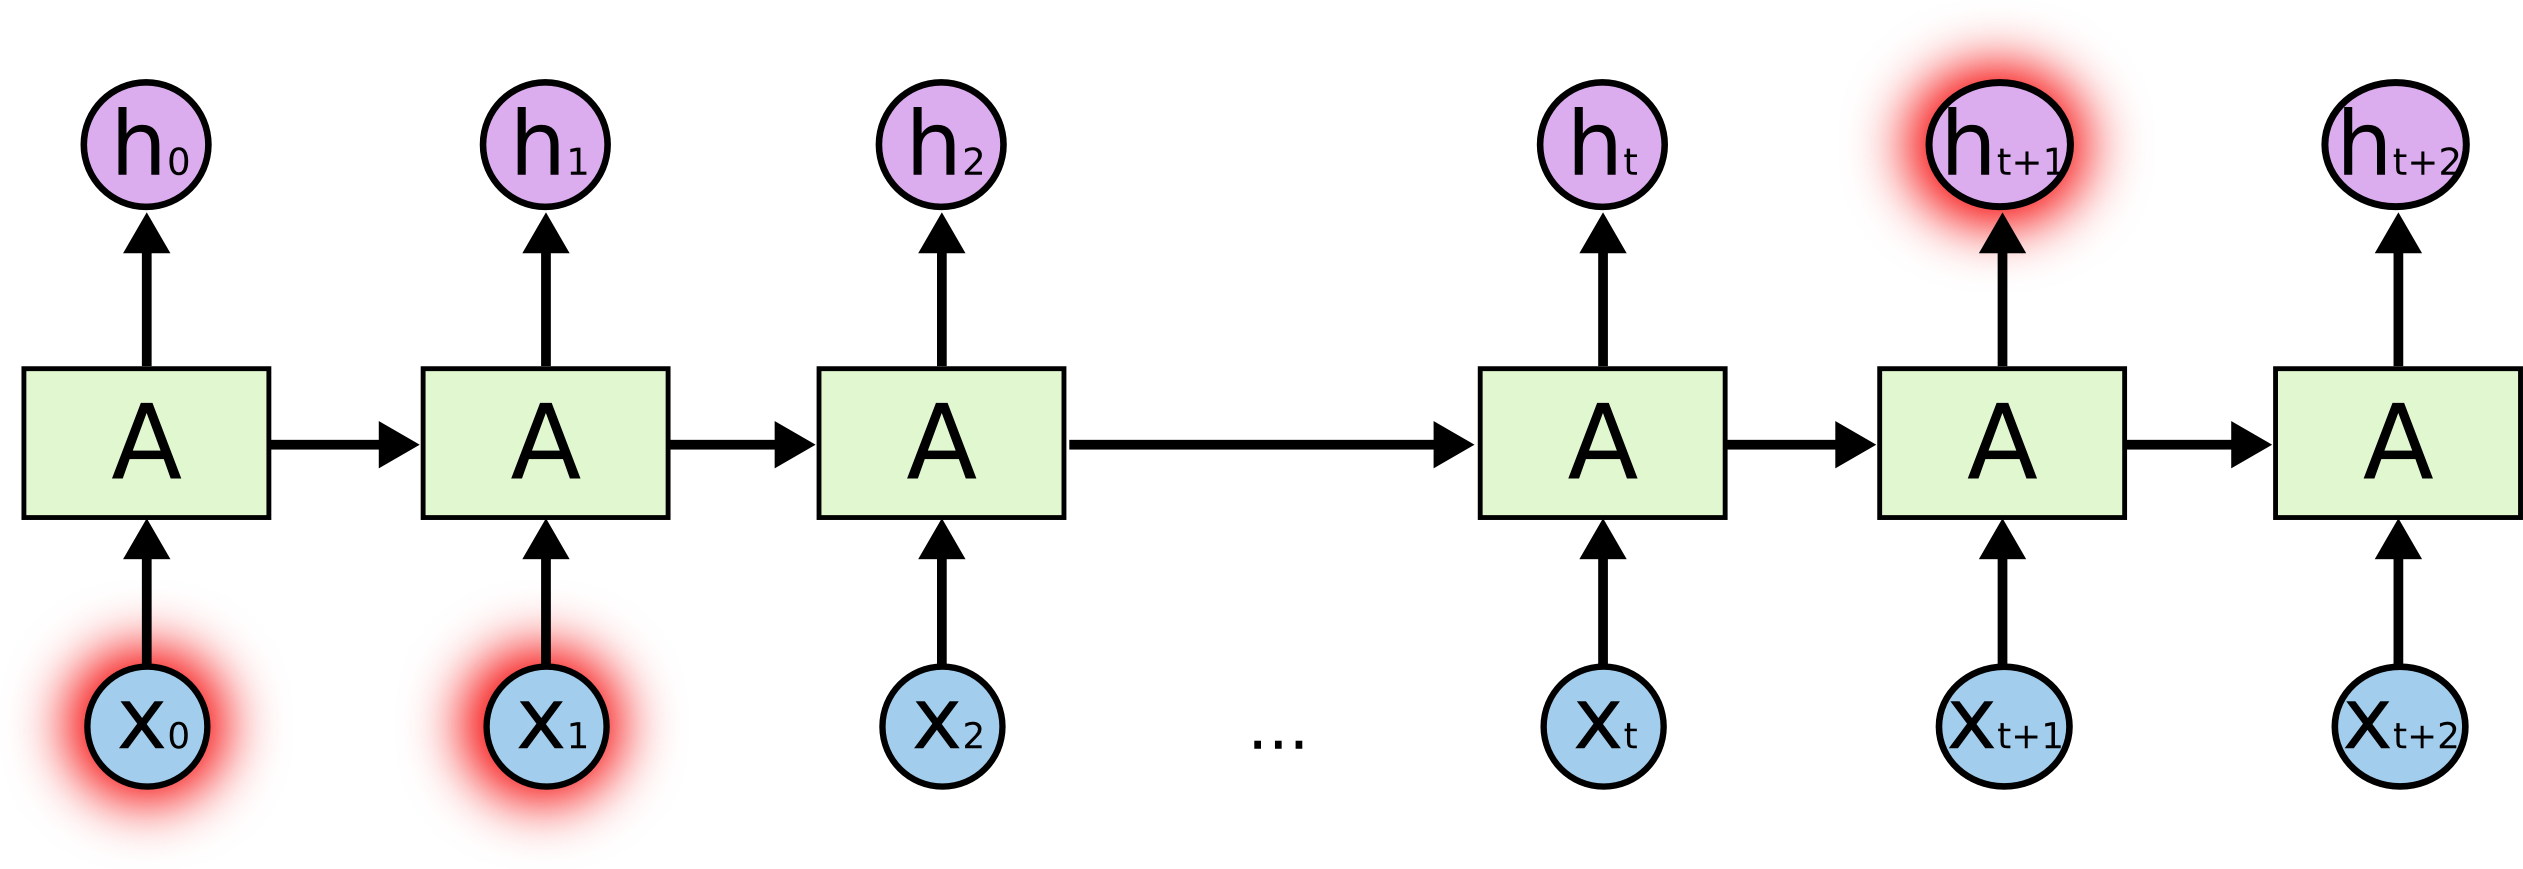
\includegraphics[width=0.9\textwidth]{RNN-longtermdependencies}}
%\caption{An unrolled recurrent neural network.}
\label{fig:rnnunrolled}
\end{figure}

In theory, RNNs are absolutely capable of handling such ``longt-term dependencies.'' A human could carefully pick parameters for them to solve toy problems of this form.  Sadly, in practice, RNNs don't seem to be able to learn them. The problem was explored in depth by  Hochreiter (1991)[German]\footnote{\url{http://people.idsia.ch/~juergen/SeppHochreiter1991ThesisAdvisorSchmidhuber.pdf}} and Bengio, et al.(1994)\footnote{\url{http://www-dsi.ing.unifi.it/~paolo/ps/tnn-94-gradient.pdf}}, who found some pretty fundamental reasons why it might be difficult.

Thankfully, LSTMs don't have this problem!

\section{LSTM Networks}

Long Short Term Memory networks---usually just called ``LSTMs''---are a special kind of RNN, capable of learning long-term dependencies. They were introduced by Hochreiter\&Schmidhuber(1997)\footnote{\url{http://deeplearning.cs.cmu.edu/pdfs/Hochreiter97\_lstm.pdf}}, and were refined and pupularized by many people in follwing work.\footnote{In addition to the original authors, a lot of people contributed to the modern LSTM. A non-comprehensive list is: Felix Gers, Fred Cummins, Santiago Fernandez, Justin Bayer, Daan Wierstra, Julian Togelius, Faustian Gomez, Matteo Gagliolo, and Alex Graves.} They work tremendously well on a large variety of problems, and are now widely used.

LSTMs are explicitly designed to avoid the long-term dependency problem. Remembering information for long periods of time is practically their default behavior, not something they struggle to learn!

All recurrent neural networks have the form of a chain of repeating modules of neural network. In standard RNNs, this repeating module will have a very simple structure, such as a single tanh layer.

\begin{figure}[H] % Example image
\center{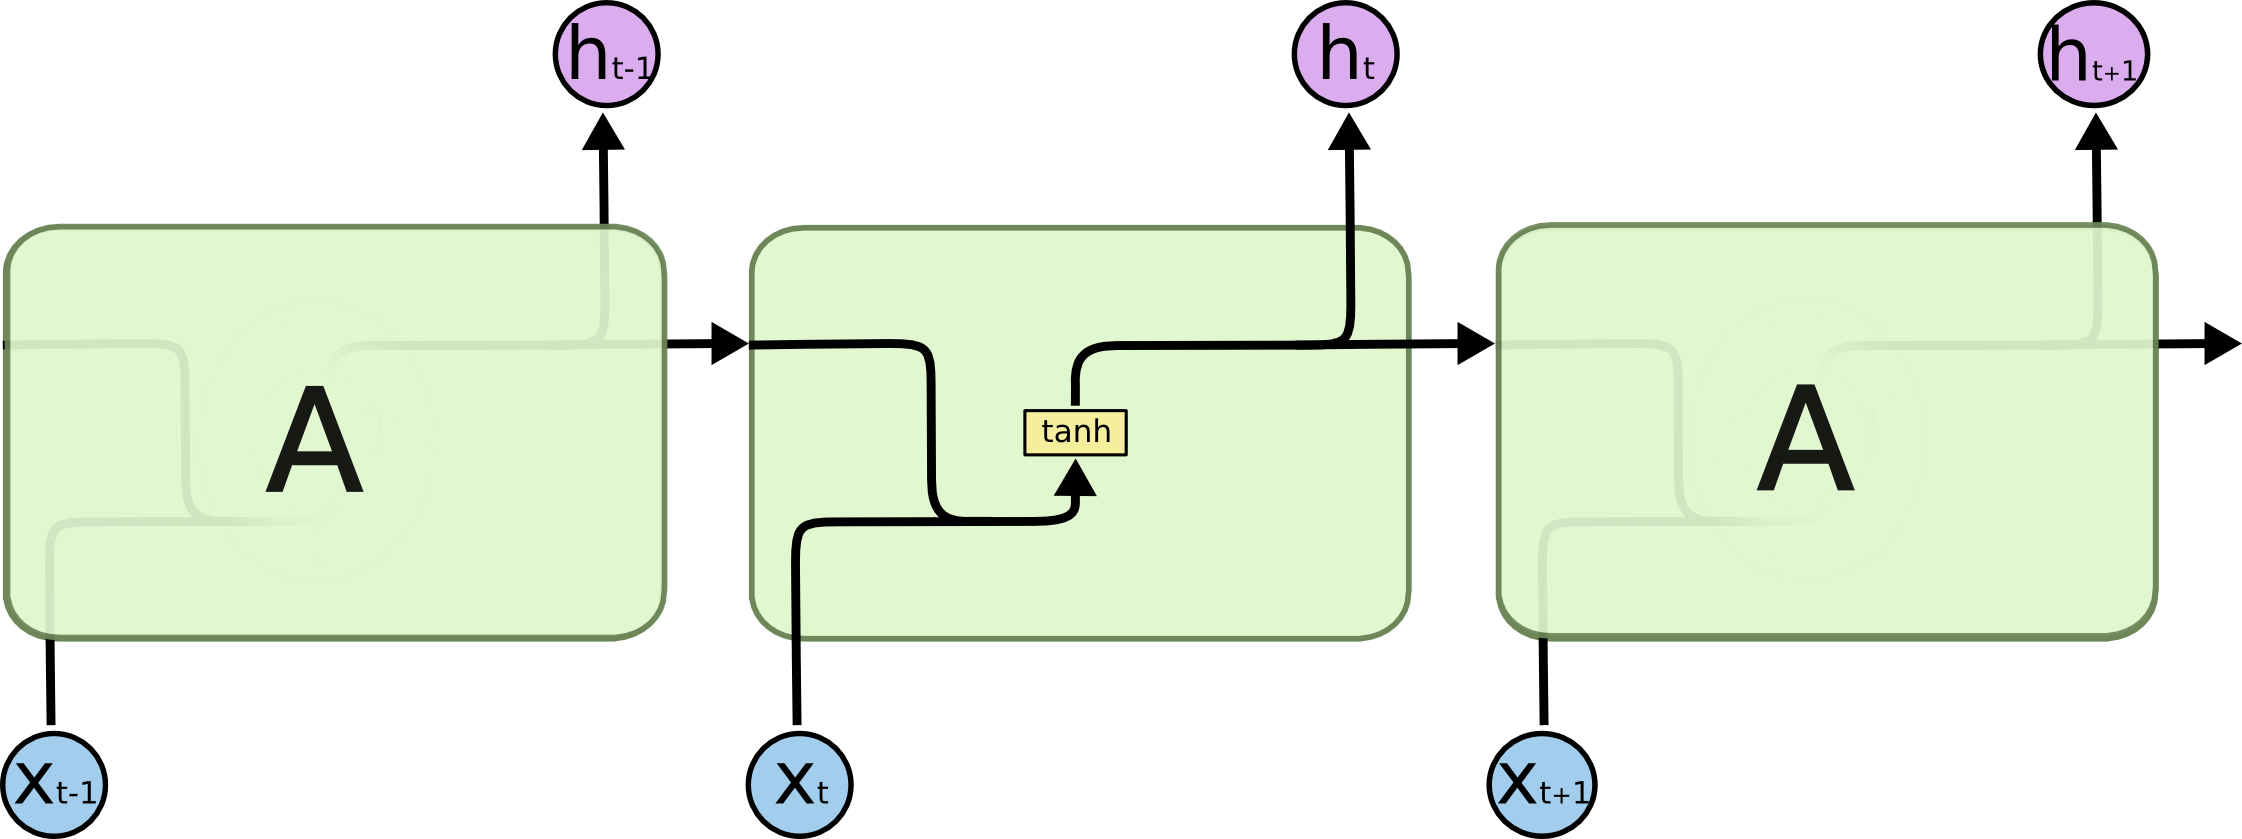
\includegraphics[width=0.9\textwidth]{LSTM3-SimpleRNN}}
\caption{The repeating module in a standard RNN contains a single layer.}
\label{fig:rnnunrolled}
\end{figure}

LSTMs also have this chain like structure, but the repeating module has a different structure. Instead of having a single neural network layer, there are four, interacting in a very special way.

\begin{figure}[H] % Example image
\center{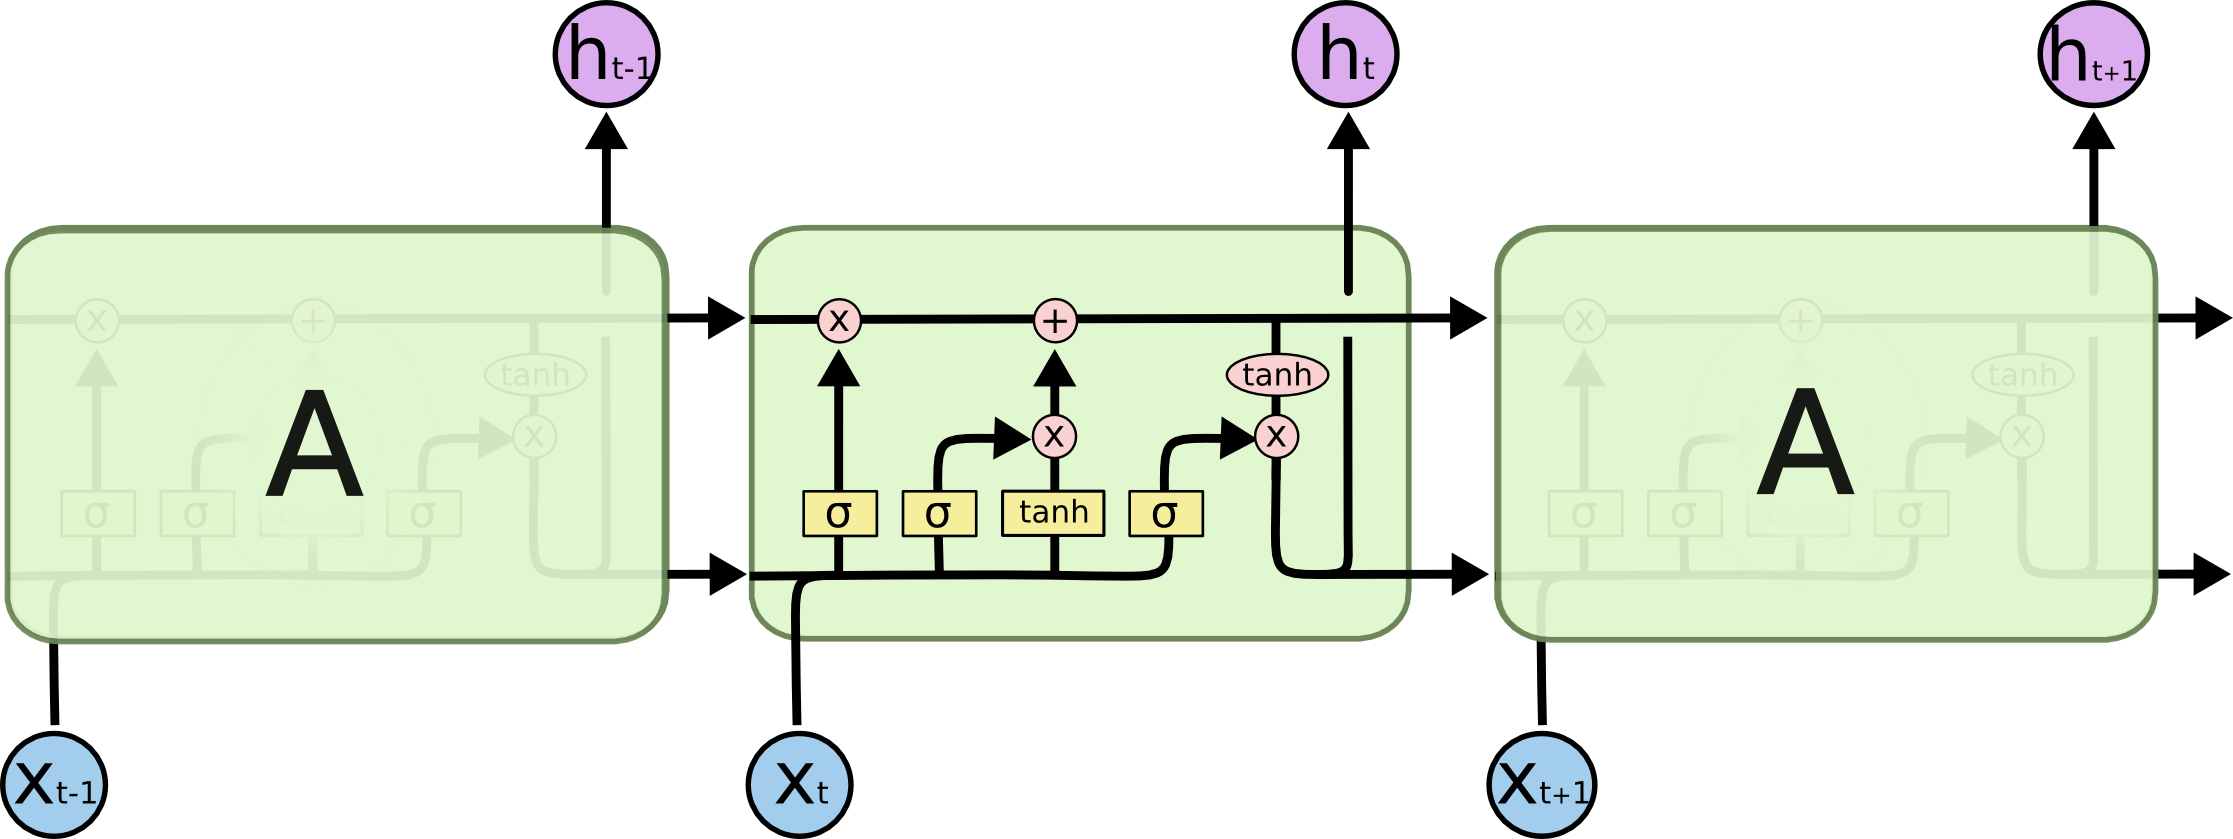
\includegraphics[width=0.9\textwidth]{LSTM3-chain}}
\caption{The repeating module in an LSTM contains four interacting layers.}
\label{fig:rnnunrolled}
\end{figure}

Don't worry about the details of what's going on. We'll walk through the LSTM diagram step by step later. For now, let's just try to get comfortable with the notation we'll be using.
%LSTM2-notation.png
\begin{figure}[H] % Example image
\center{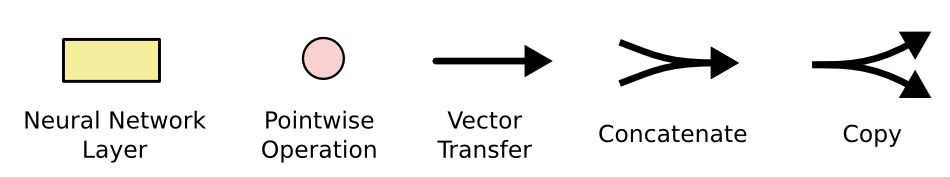
\includegraphics[width=0.9\textwidth]{LSTM2-notation}}
%\caption{.}
\label{fig:rnnunrolled}
\end{figure}

In the above diagram, each line carries an entire vector, from the output of one node to the inputs of others. The pink circles represent pointwise operations, like vector addition, while the yello boxes are learned neural network layers. Lines merging denote concatenation, while a line forking denote its content being copied and the copies going to different locations.

\section{The Core Idea Behind LSTMs}

The key to LSTMs is the cell state, the horizontal line running through the top of the diagram.

The cell state is kind of like a conveyor belt. It runs straight down the entire chain, with only some minor linear interactions. It's very easy for information to just flow along it unchanged.
%LSTM3-C-line.png
\begin{figure}[H] % Example image
\center{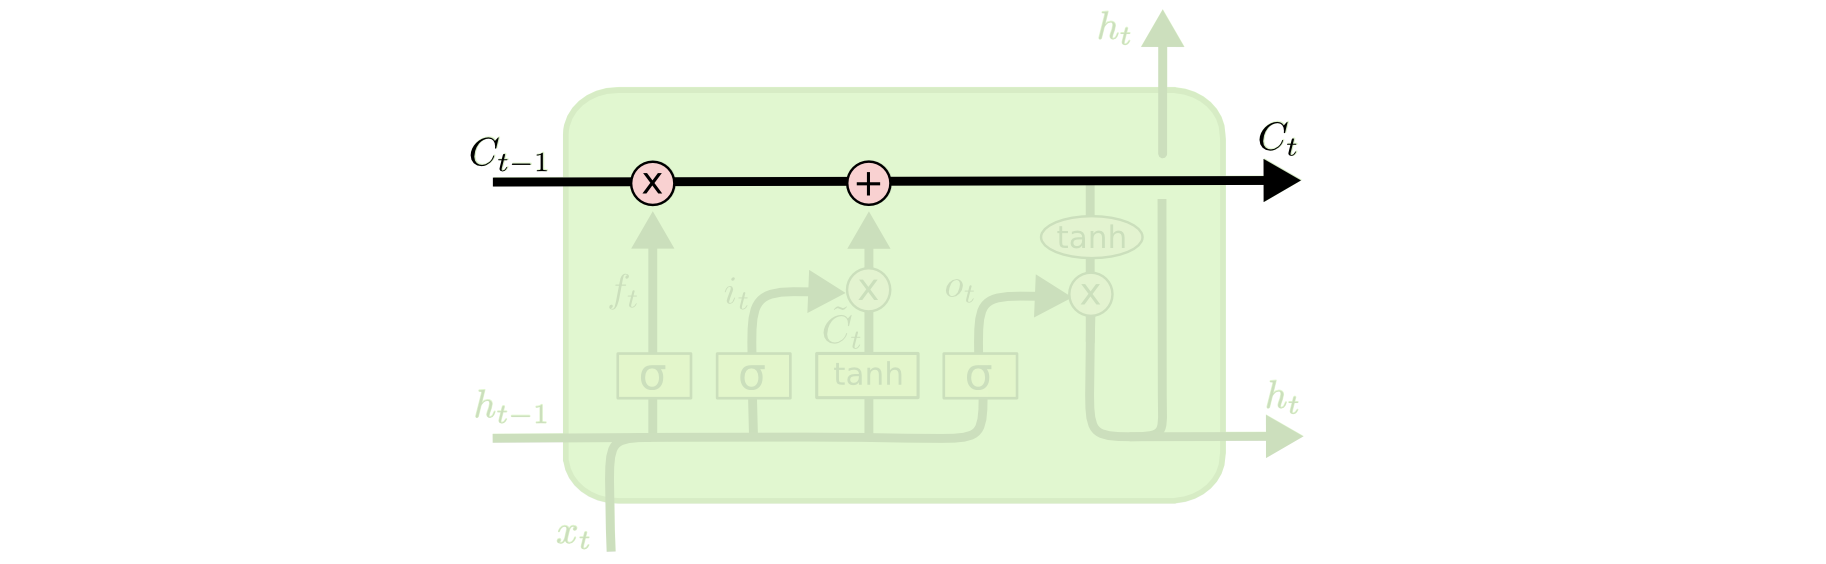
\includegraphics[width=0.9\textwidth]{LSTM3-C-line}}
%\caption{.}
\label{fig:rnnunrolled}
\end{figure}

The LSTM does have the ability to remove or add information to the cell state, carefully regulated by structures called gates.

Gates are a way to optionally let information through. They are composed out of a sigmoid neural net layer and a pointwise multiplication operation.
%LSTM3-gate.png
\begin{figure}[H] % Example image
\center{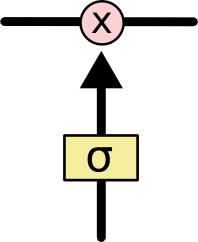
\includegraphics[width=0.2\textwidth]{LSTM3-gate}}
%\caption{.}
\label{fig:rnnunrolled}
\end{figure}

The sigmoid layer outputs numbers between zero and one, describing how much of each component should be let through. A value of zero means ``let nothing through,'' while a value of one means ``let everything through!''

An LSTM has three of these gates, to protect and control the cell state.

\section{Step-by-Step LSTM Walk Through}

The first step in our LSTM is to decide what information we're going to throw away from the cell state. This decision is made by a sigmoid layer called the ``forget gate layer.'' It looks at $h_{t-1}$ and $x_{t}$, and outputs a number between 0 and 1 for each number in the cell state $C_{t-1}$. A 1 represents ``completely keep this'' while a 0 represents ``completely get rid of this.''

Let's go back to our example of a language model trying to predict the next word based on all the previous ones. In such a problem, the cell state might include the gender of the present subject, so that the correct pronouns can be used. When we see a new subject, we want to forget the gender of the old subject.
%LSTM3-focus-f.png
\begin{figure}[H] % Example image
\center{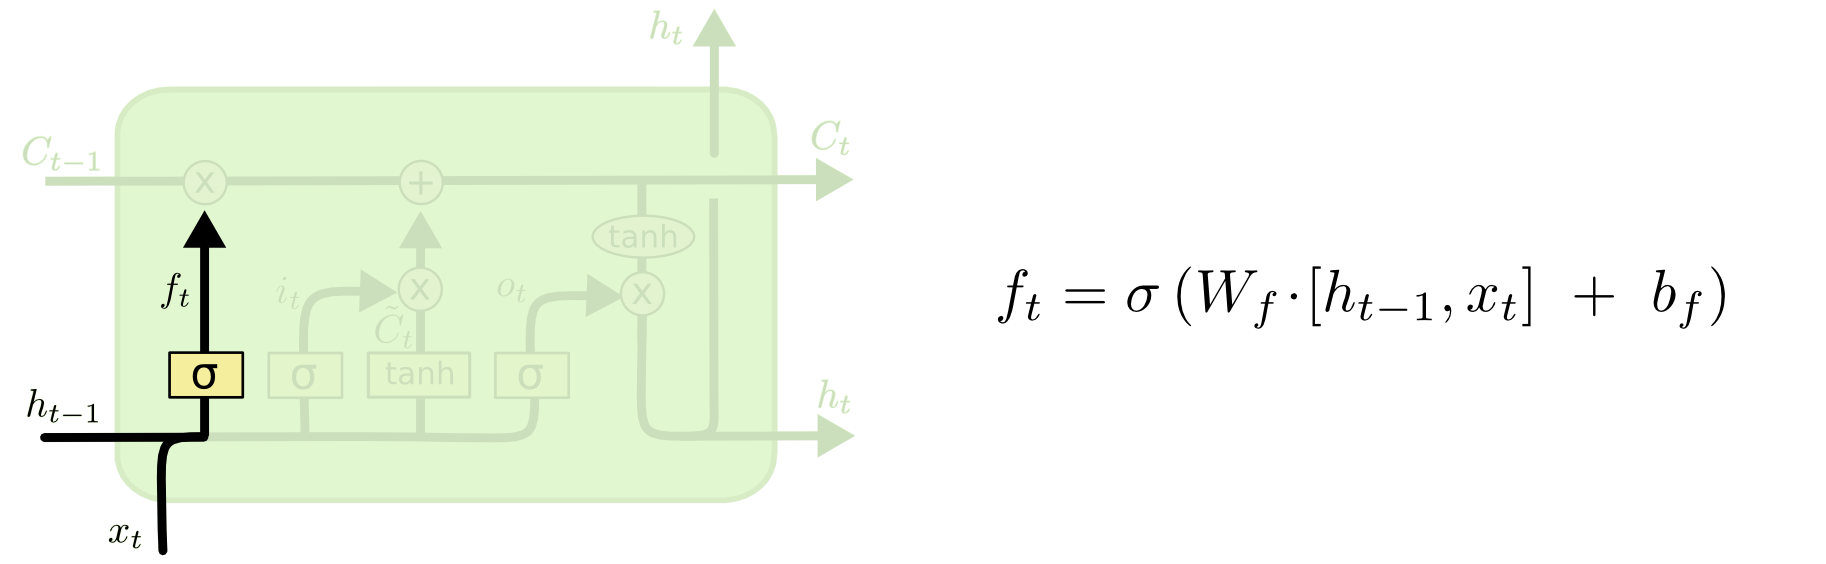
\includegraphics[width=0.9\textwidth]{LSTM3-focus-f}}
%\caption{.}
\label{fig:rnnunrolled}
\end{figure}

The next step is to decide what new information we're going to store in the cell state. This has two parts. First, a sgimoid layer called the ``input gate layer'' decides which values we'll update. Next, a tanh layer creates a vector of new candidate values, $\tilde{C}_{t}$, that could be added to the state. In the next step, we'll combine these two to create an update to the state.

In the example of our language model, we'd want to add the gender of the new subject to the cell state, to replace the old one we're forgetting.

\begin{figure}[H] % Example image
\center{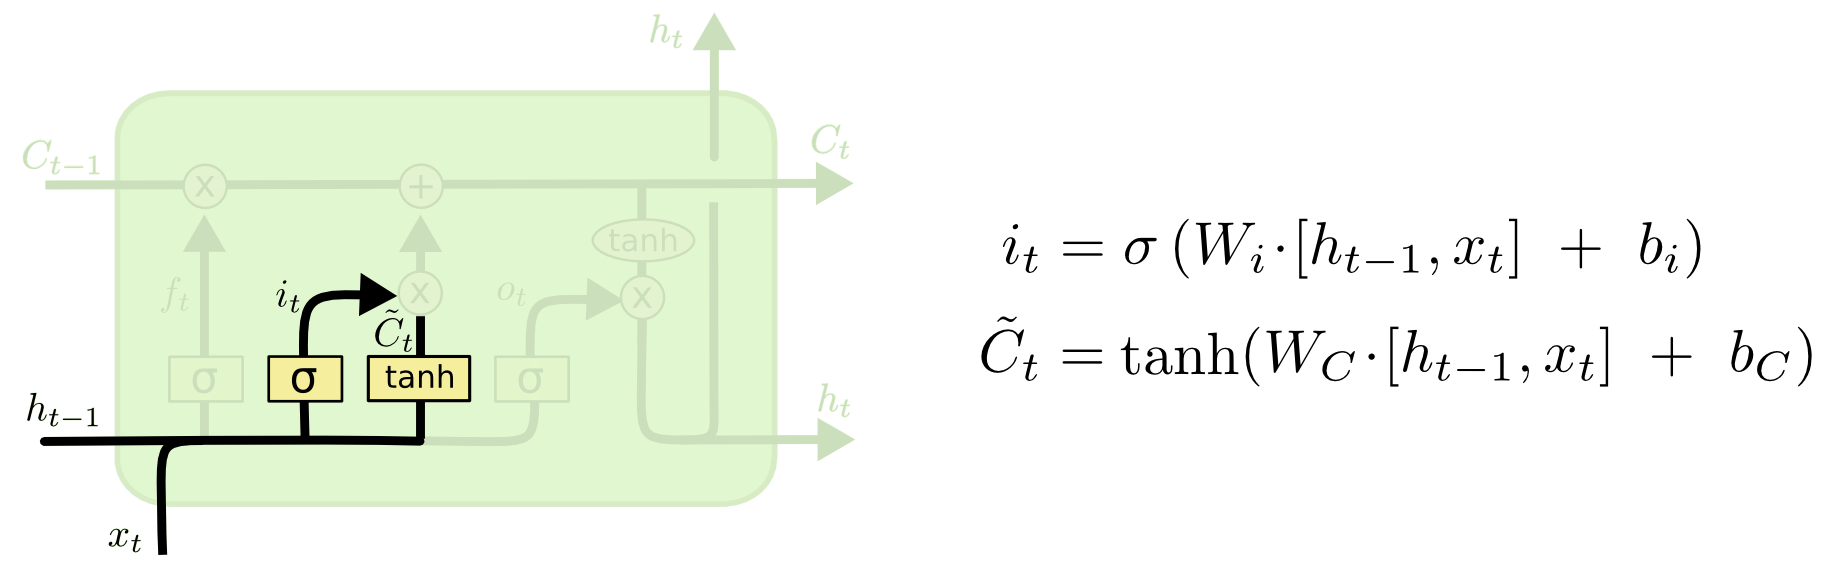
\includegraphics[width=0.9\textwidth]{LSTM3-focus-i}}
%\caption{.}
\label{fig:rnnunrolled}
\end{figure}

It's now time to update the old cell state, $C_{t-1}$, into the new cell state $C_{t}$. The previous steps already decided what to do, we just need to actually do it.

We multiply the old state by $f_{t}$, forgetting the things we dicided to forget earlier. Then we add $i_{t}*\tilde{C}_{t}$. This is the new candidate values, scaled by how much we decide to update each state value.

In the case of the language model, this is where we'd actually drop the information about the old subject's gender and add the new information, as we decided in the previous steps.

\begin{figure}[H] % Example image
\center{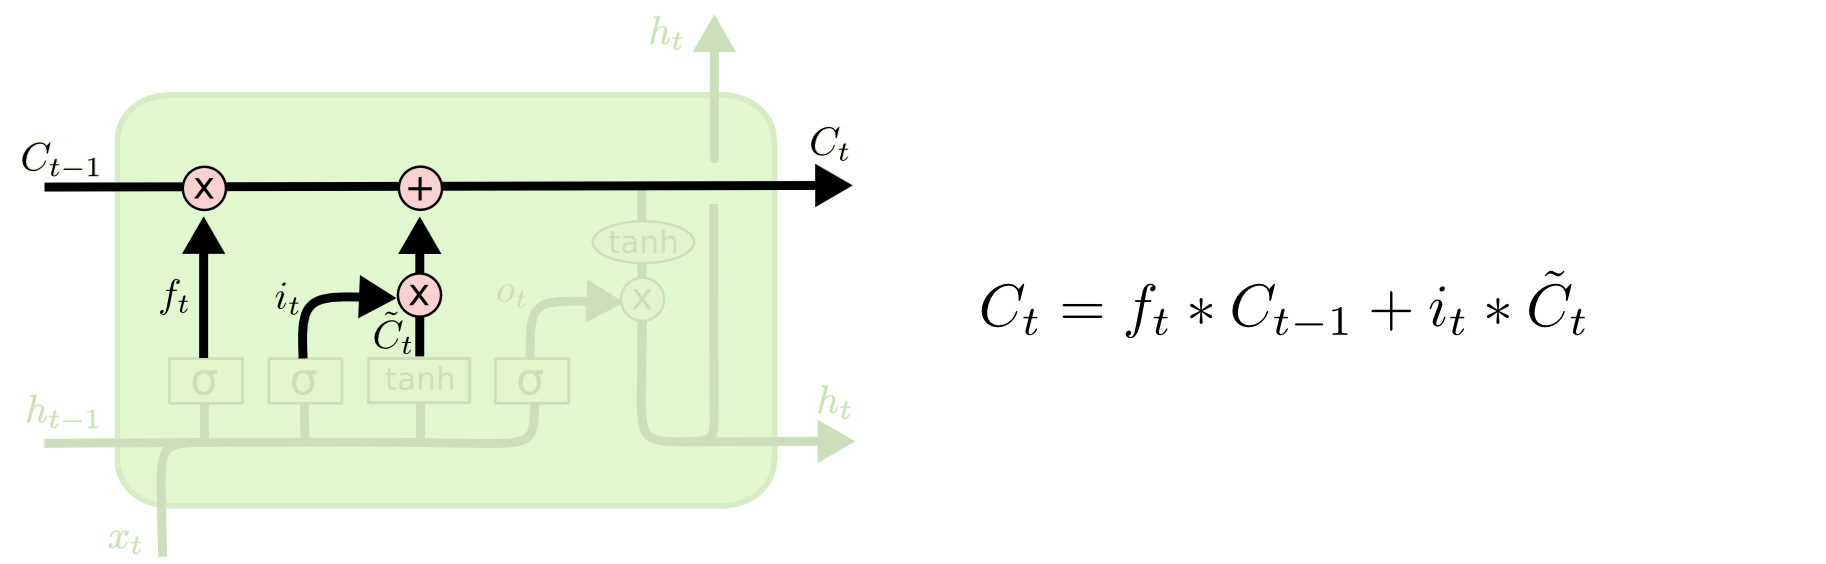
\includegraphics[width=0.9\textwidth]{LSTM3-focus-C}}
%\caption{.}
\label{fig:rnnunrolled}
\end{figure}

Finally, we need to decide what we're going to output. This output will be based on our cell state, but will be a filtered version. First, we run a sigmoid layer which decides what parts of the cell state we're going to output. Then, we put the cell state through tanh (to push the values to be between -1 and 1) and multiply it by the output of the sigmoid gate, so that we only output the parts we decided to.

For the language model example, since it just saw a subject, it might want to output information relevant to a verb, in case that's what is coming next. For example, it might output whether the subject is singular or plural, so that we know what form a verb should be conjugated into if that's what follows next.

\begin{figure}[H] % Example image
\center{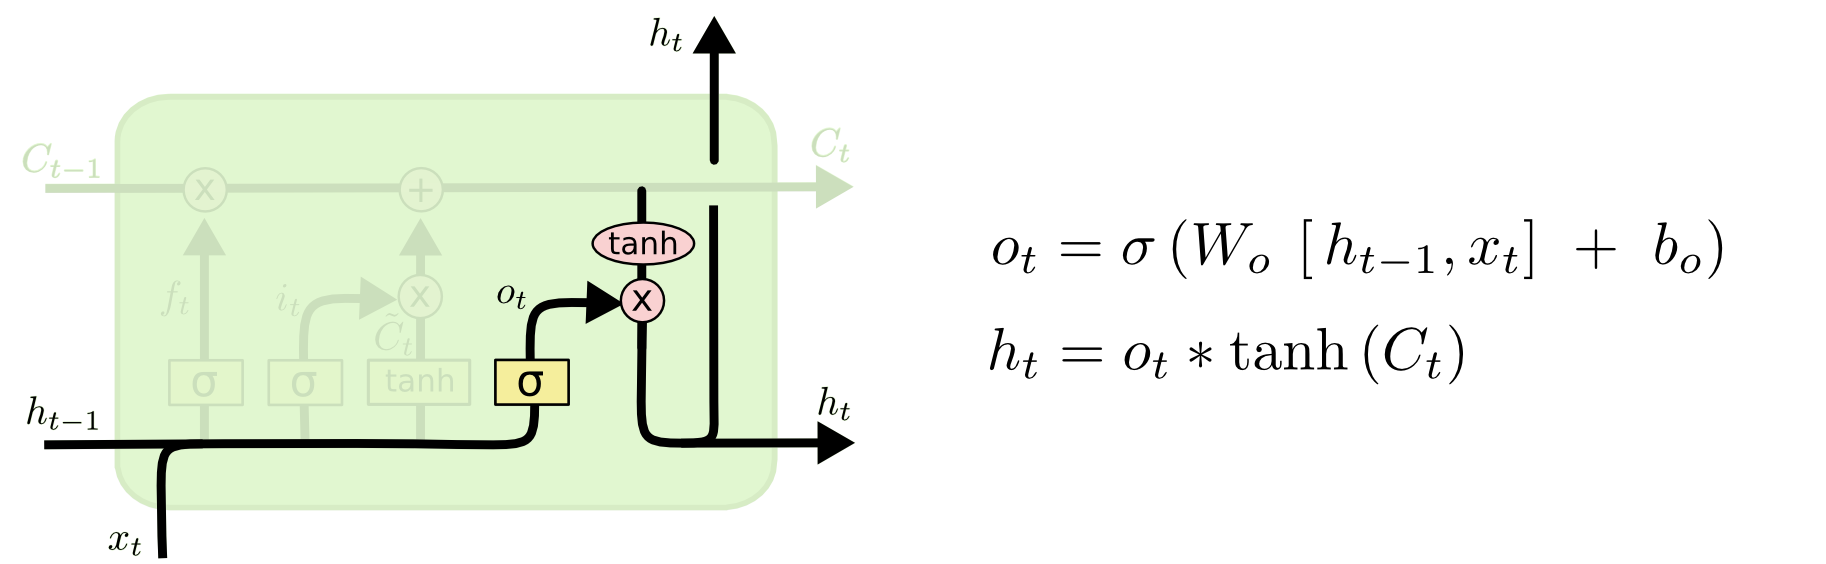
\includegraphics[width=0.9\textwidth]{LSTM3-focus-o}}
%\caption{.}
\label{fig:rnnunrolled}
\end{figure}

\section{Variants on Long Short Term Memory}

What I've described so far is a pretty normal LSTM. But not all LSTMs are the same as the above. In fact, it seems like almost every paper involving LSTMs uses a slightly different version. The differences are minor, but it's worth mentioning some of them.

One popular LSTM variant, introduced by Gers \& Schmidhuber (2000)\footnote{\url{ftp://ftp.idsia.ch/pub/juergen/TimeCount-IJCNN2000.pdf}}, is adding ``peephole connections.'' This means that we let the gate layers look at the cell state.

%LSTM3-var-peepholes.png
\begin{figure}[H] % Example image
\center{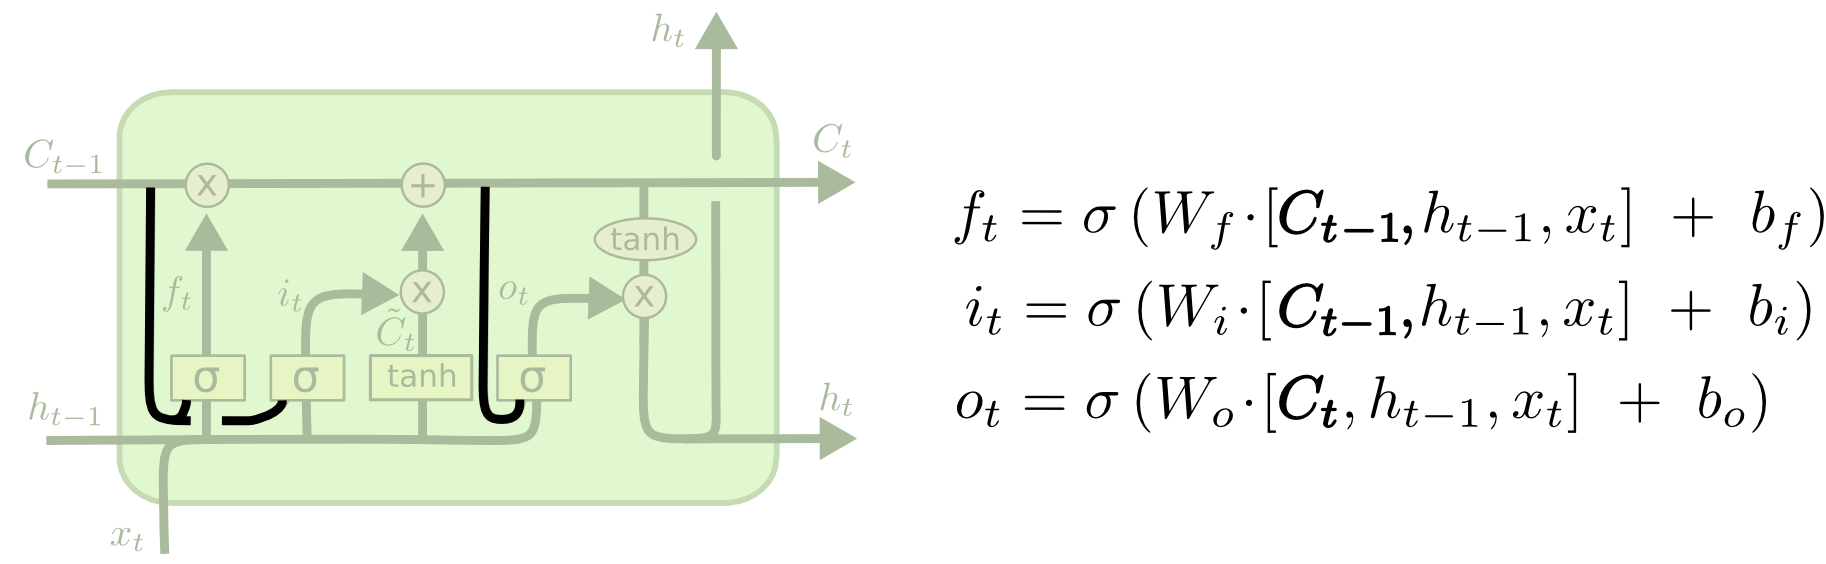
\includegraphics[width=0.9\textwidth]{LSTM3-var-peepholes}}
%\caption{.}
\label{fig:rnnunrolled}
\end{figure}

This above diagram adds peepholes to all the gates, but many papers will give some peepholes and not others.

Another variation is to use coupled forget and input gates. Instead of separately deciding what to forget and what we should add new information to, we make those decisions together. We only forget when we're going to input something in its place. We only input new values to the state when we forget something older.
%LSTM3-var-tied.png
\begin{figure}[H] % Example image
\center{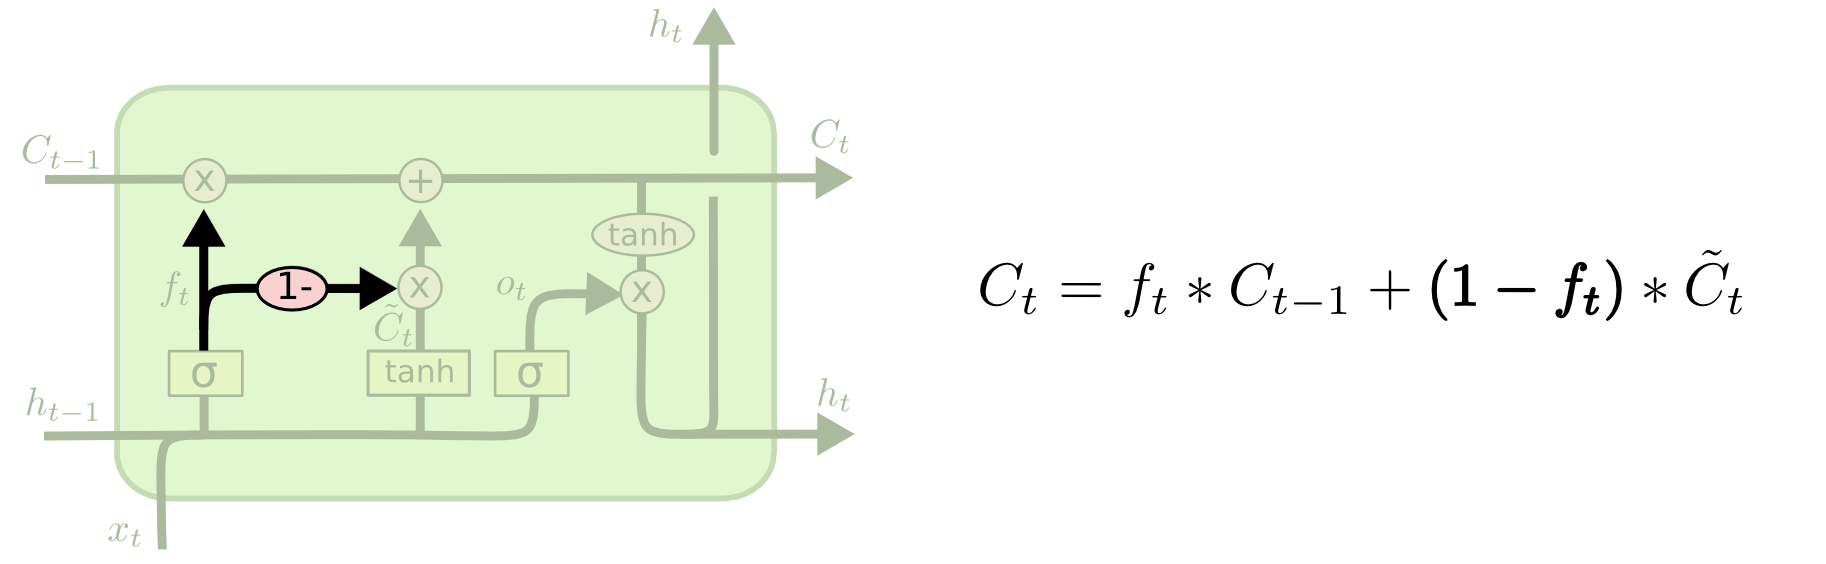
\includegraphics[width=0.9\textwidth]{LSTM3-var-tied}}
%\caption{.}
\label{fig:rnnunrolled}
\end{figure}

A slightly more dramatic variation on the LSTM is the Gated Recurrent Unit, of GRU, introduced by Cho, et al.(2014)\footnote{\url{http://arxiv.org/pdf/1406.1078v3.pdf}}. It combines the forge and input gates into a single ``update gate.'' It also merges the cell state and hidden state, and makes some other changes. The resulting model is simpler than standard LSTM models, and has been growing increasingly popular.

\begin{figure}[H] % Example image
\center{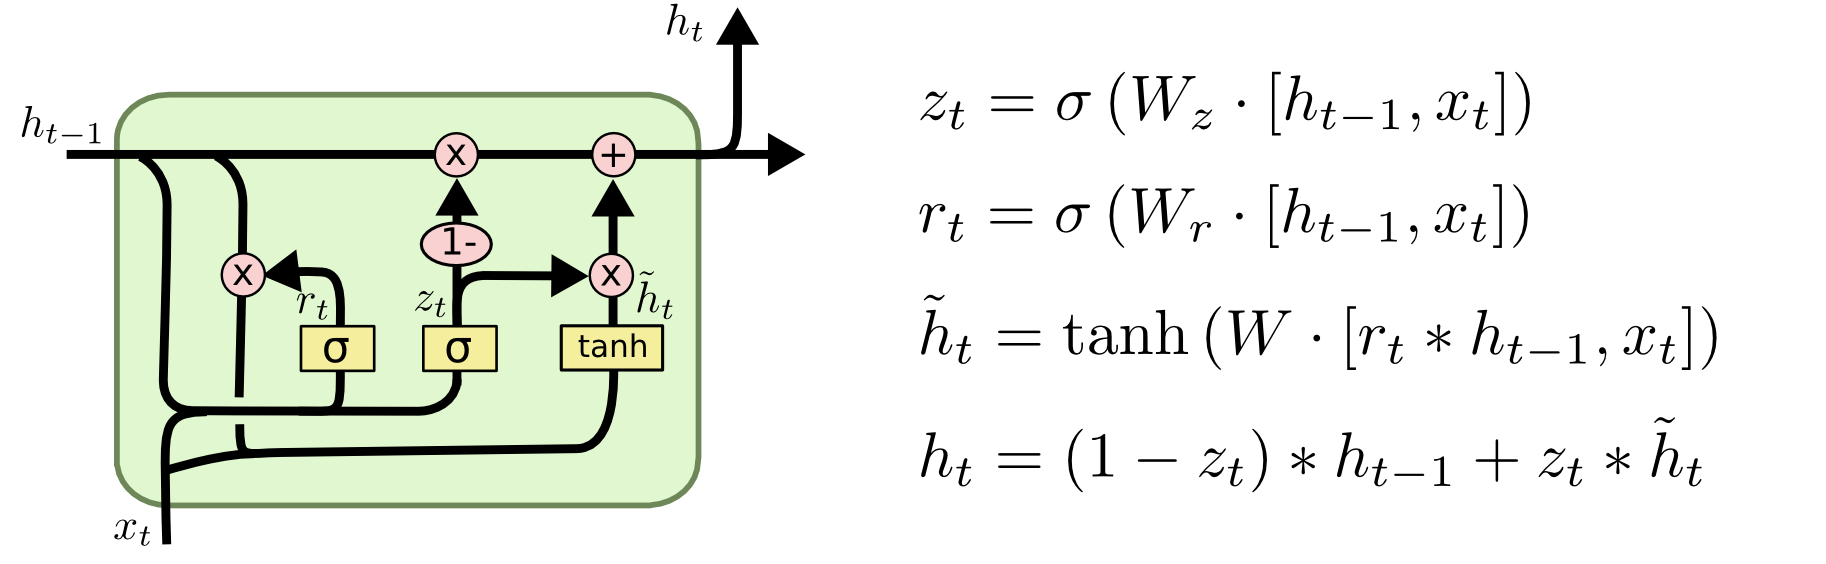
\includegraphics[width=0.9\textwidth]{LSTM3-var-GRU}}
%\caption{.}
\label{fig:rnnunrolled}
\end{figure}

These are only a few of the most notable LSTM variants. There are lots of others, like Depth Gated RNNs by Yao, et al.(2015)\footnote{\url{http://arxiv.org/pdf/1508.03790v2.pdf}}. There's also some completely different approach to tackling long-term dependencies, like Clockwork RNNs by Koutnik, et al. (2014).\footnote{\url{http://arxiv.org/pdf/1402.3511v1.pdf}}

Which of these variants is best? Do the differences matter? Greff, et al. (2015)\footnote{\url{http://arxiv.org/pdf/1503.04069.pdf}} do a nice comparison of popular variants, finding that they're all about the same. Jozefowice, et al. (2015)\footnote{\url{http://jmlr.org/proceedings/papers/v37/jozefowicz15.pdf}} tested more than ten thousand RNN architectures, finding some that worked better than LSTMs on certain tasks.

\section{Conclusion}

Earlier, I mentioned the remarkable results people are achieving with RNNs. Essentially all of these are achieved using LSTMs. They really work a lot better for most tasks!

Written down as a set of equations, LSTMs look pretty intimidating. Hopefully, walking through them step by step in this essay has made them a bit more approachable.

LSTMs were a big step in what we can accomplish with RNNs. It's natural to wonder: is there another big step? A common opinion among researchers is :''Yes! There is a next step and it's attention!'' The idea is to let every step of an RNN pick information to look at from some larger collection of information. For example, if you are using an RNN to create a caption describing an image, it might pick a part of the image to look at for every word it outputs. In fact, Xu, et al. (2015)\footnote{\url{http://arxiv.org/pdf/1502.03044v2.pdf}} do exactly this---it might be a fun starting point if you want to explore attention! There's been a number of really exciting results using attention, and it seems like a lot more are around the corner...

Attention isn't the only exciting thread in RNN research. For example, Grid LSTMs by Kalchbrenner, et al. (2015)\footnote{\url{http://arxiv.org/pdf/1507.01526v1.pdf}} seem extremely promising. Work using RNNs is generative models---such as Gregor, et al. (2015)\footnote{\url{http://arxiv.org/pdf/1502.04623.pdf}}, Chung, et al. (2015)\footnote{\url{http://arxiv.org/pdf/1506.02216v3.pdf}}, or Bayere \& Osendorfer (2015)\footnote{\url{http://arxiv.org/pdf/1411.7610v3.pdf}} --- also seems very interesting. The last few years have been an exciting time for recurrent neural networks, and the coming ones promise to only be more so!

\section{Acknowledgments}

I'm grateful to a number of people for helping me better understanding LSTMs, commenting on the visualizations, and providing feedback on this post.

I'm very grateful to my colleagues at Google for their helpful feedback, especially Oriol Vinyals, Greg Corrado, Jon Shlens, Luke Vilnis, and Ilya Sutskever. I'm also thankful to many other friends and colleagues for taking the time to help me, including Dario Amodei, and Jacob Steinhardt. I'm especially thankful to Kyunghyun Cho for extremely thoughtful correspondence about my diagrams.

Before this post, I practiced explaining LSTMs during two seminar series I taught on neural networks. Thanks to everyone who participated in those for their patience with me, and for their feedback.



%-------------------------------------------------------------------

\end{document}